%--------------------------------------------------------------------------------
% Constrói a capa com base na seção de identificação do main.tex
%--------------------------------------------------------------------------------
\begin{capa}
    \setlength{\belowcaptionskip}{0pt}
    \setlength{\abovecaptionskip}{0pt}
    \setlength{\intextsep}{-18pt}
        \begin{figure}[h]
    		\begin{center}
    		    
\includegraphics[scale=1.0]{img/LOGO_UNIVASF_big.pdf}
    		\end{center}
    	\end{figure}

        %
\includegraphics[scale=0.6]{img/univasf.jpg}
        \center
    	{\ABNTEXchapterfont\large\imprimirinstituicao}

    	\vspace*{2cm}
    	    {\imprimirautor}
    	\vspace*{2cm}
    %	\vfill
        \begin{center}
    		\ABNTEXchapterfont\bfseries\large\imprimirtitulo
        \end{center}
    	\vfill

    	\ABNTEXchapterfont\bfseries\large\imprimirlocal\\ 
    	\the\year

    	\vspace*{1cm}
\end{capa}
%--------------------------------------------------------------------------------
% Constrói a folha de rosto com base na seção de identificação do main.tex
%--------------------------------------------------------------------------------
\begin{folhaderosto}
\center
    	{\ABNTEXchapterfont\large\imprimirinstituicao}

		\vspace*{2cm}
    	    {\imprimirautor}
    	\vspace*{2cm}
		\vspace*{\fill}

		{\ABNTEXchapterfont\bfseries\large\imprimirtitulo}
		\vspace*{\fill}

		{\hspace{.45\textwidth}
		\begin{minipage}{.5\textwidth}
			\SingleSpacing
			\imprimirpreambulo \\ \\

			{\imprimirorientadorRotulo~\imprimirorientador\par}
			{\imprimircoorientadorRotulo~\imprimircoorientador\par}

		\end{minipage}%
		\vspace*{\fill}}%
		\vspace*{\fill}
			\ABNTEXchapterfont\bfseries\large\imprimirlocal\\ 
			\the\year
		\vspace*{1cm}
\end{folhaderosto}

%--------------------------------------------------------------------------------
% Constrói a ficha catalográfia com base na seção de identificação do main.tex
% Está comentado porque no final das contas a biblioteca do seu campus que gera a 
% numeração, você pode adicionar os numeros aqui, ou anexar o pdf gerado por eles
% ao documento.
%--------------------------------------------------------------------------------
%\begin{fichacatalografica}
%	\vspace*{\fill}					% Posição vertical
%	\hrule							% Linha horizontal
%	\begin{center}					% Minipage Centralizado
%	\begin{minipage}[c]{12.5cm}		% Largura
%
%	\imprimirautor
%
%	\hspace{0.5cm} \imprimirtitulo  / \imprimirautor. --
%	\imprimirlocal, \the\year-
%
%	\hspace{0.5cm} xx p. : il. (algumas color.) ; 30 cm.\\
%
%	\hspace{0.5cm} \imprimirorientadorRotulo~\imprimirorientador\\
%
%	\hspace{0.5cm}
%	\parbox[t]{\textwidth}{\imprimirtipotrabalho~--~\imprimirinstituicao,
%	\the\year.}\\
%
%	\hspace{0.5cm}
%		1. Palavra-chave1.
%		2. Palavra-chave2.
%		I. Orientador.
%		II. Universidade xxx.
%		III. Faculdade de xxx.
%		IV. Título\\
%
%	\hspace{8.75cm} CDU 02:141:005.7\\
%
%	\end{minipage}
%	\end{center}
%	\hrule
%\end{fichacatalografica}

%--------------------------------------------------------------------------------
% Anexando a ficha catalogáfica e a folha de aprovação 
%--------------------------------------------------------------------------------
%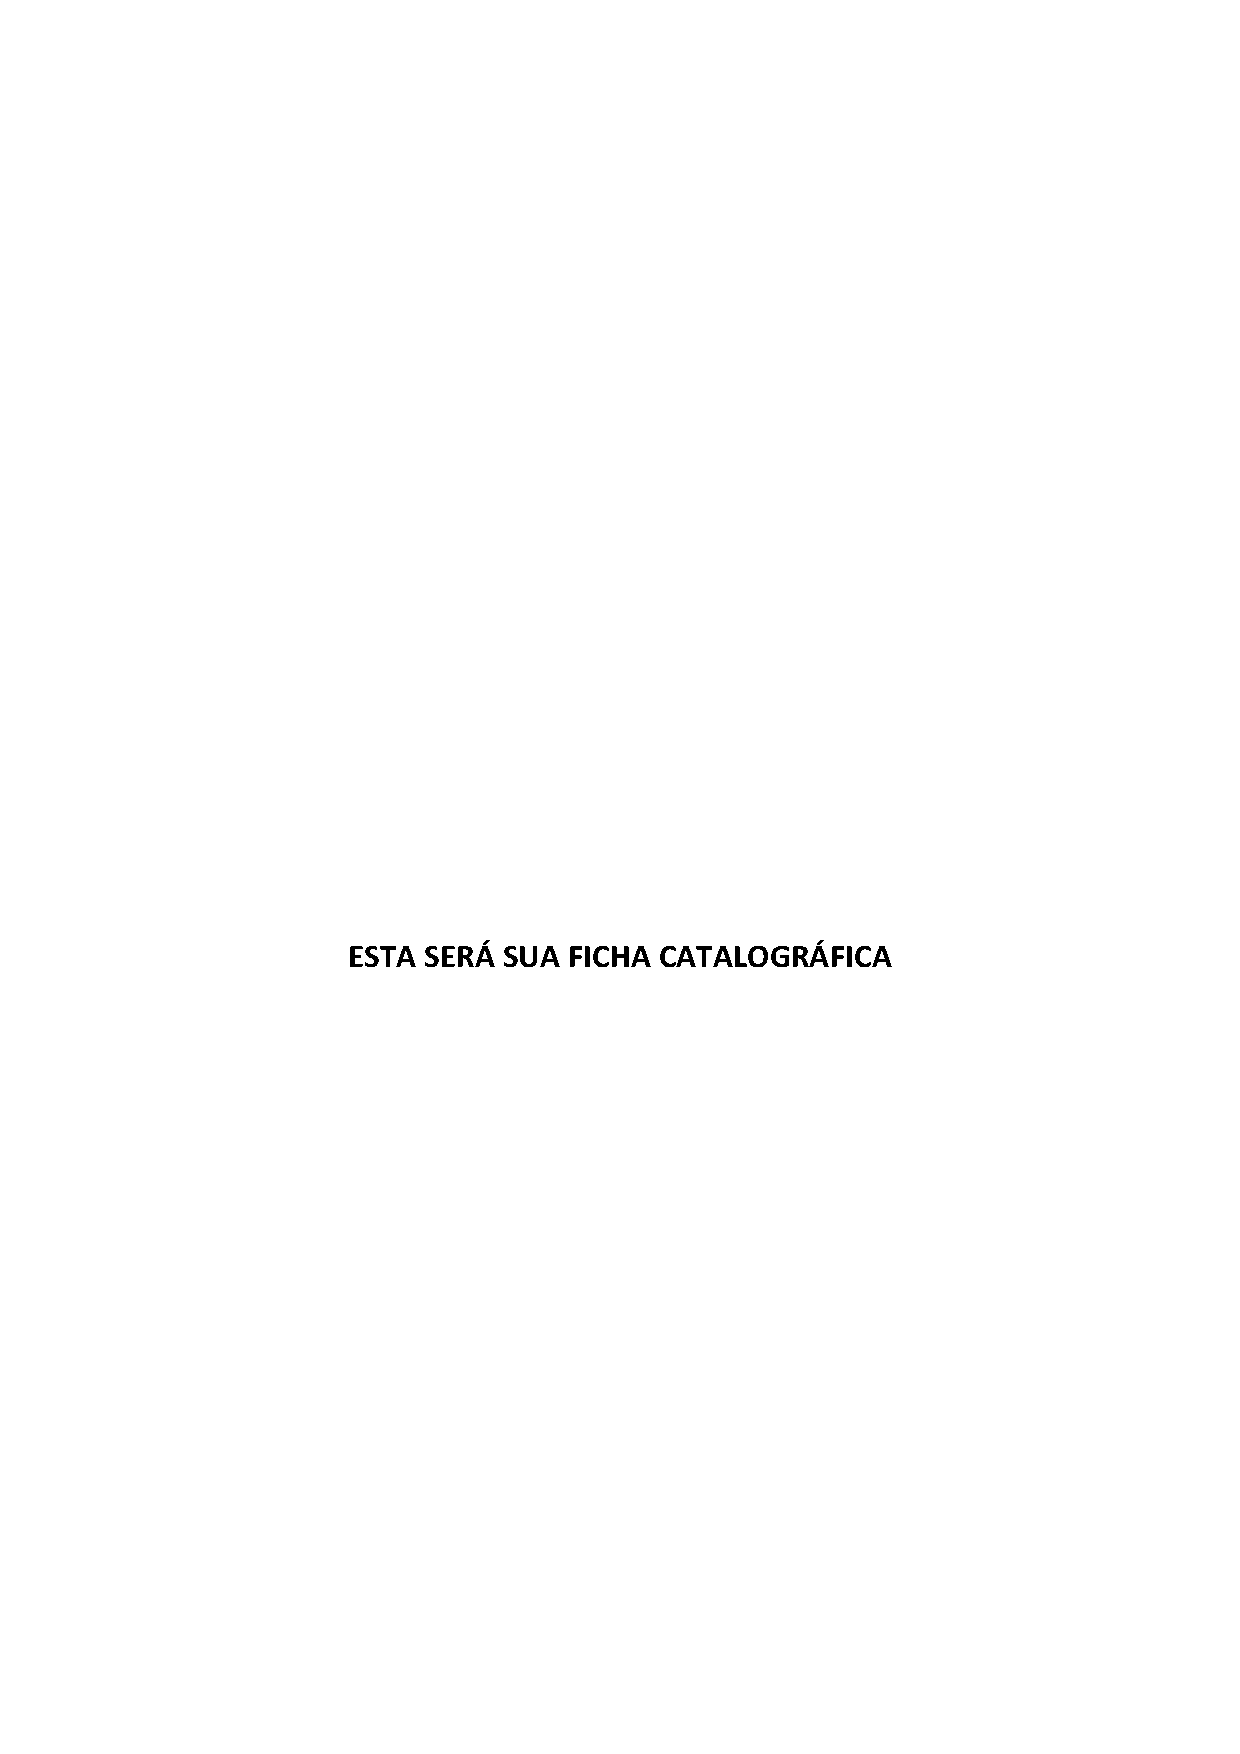
\includepdf[pages=-]{anexos/ficha.pdf}

%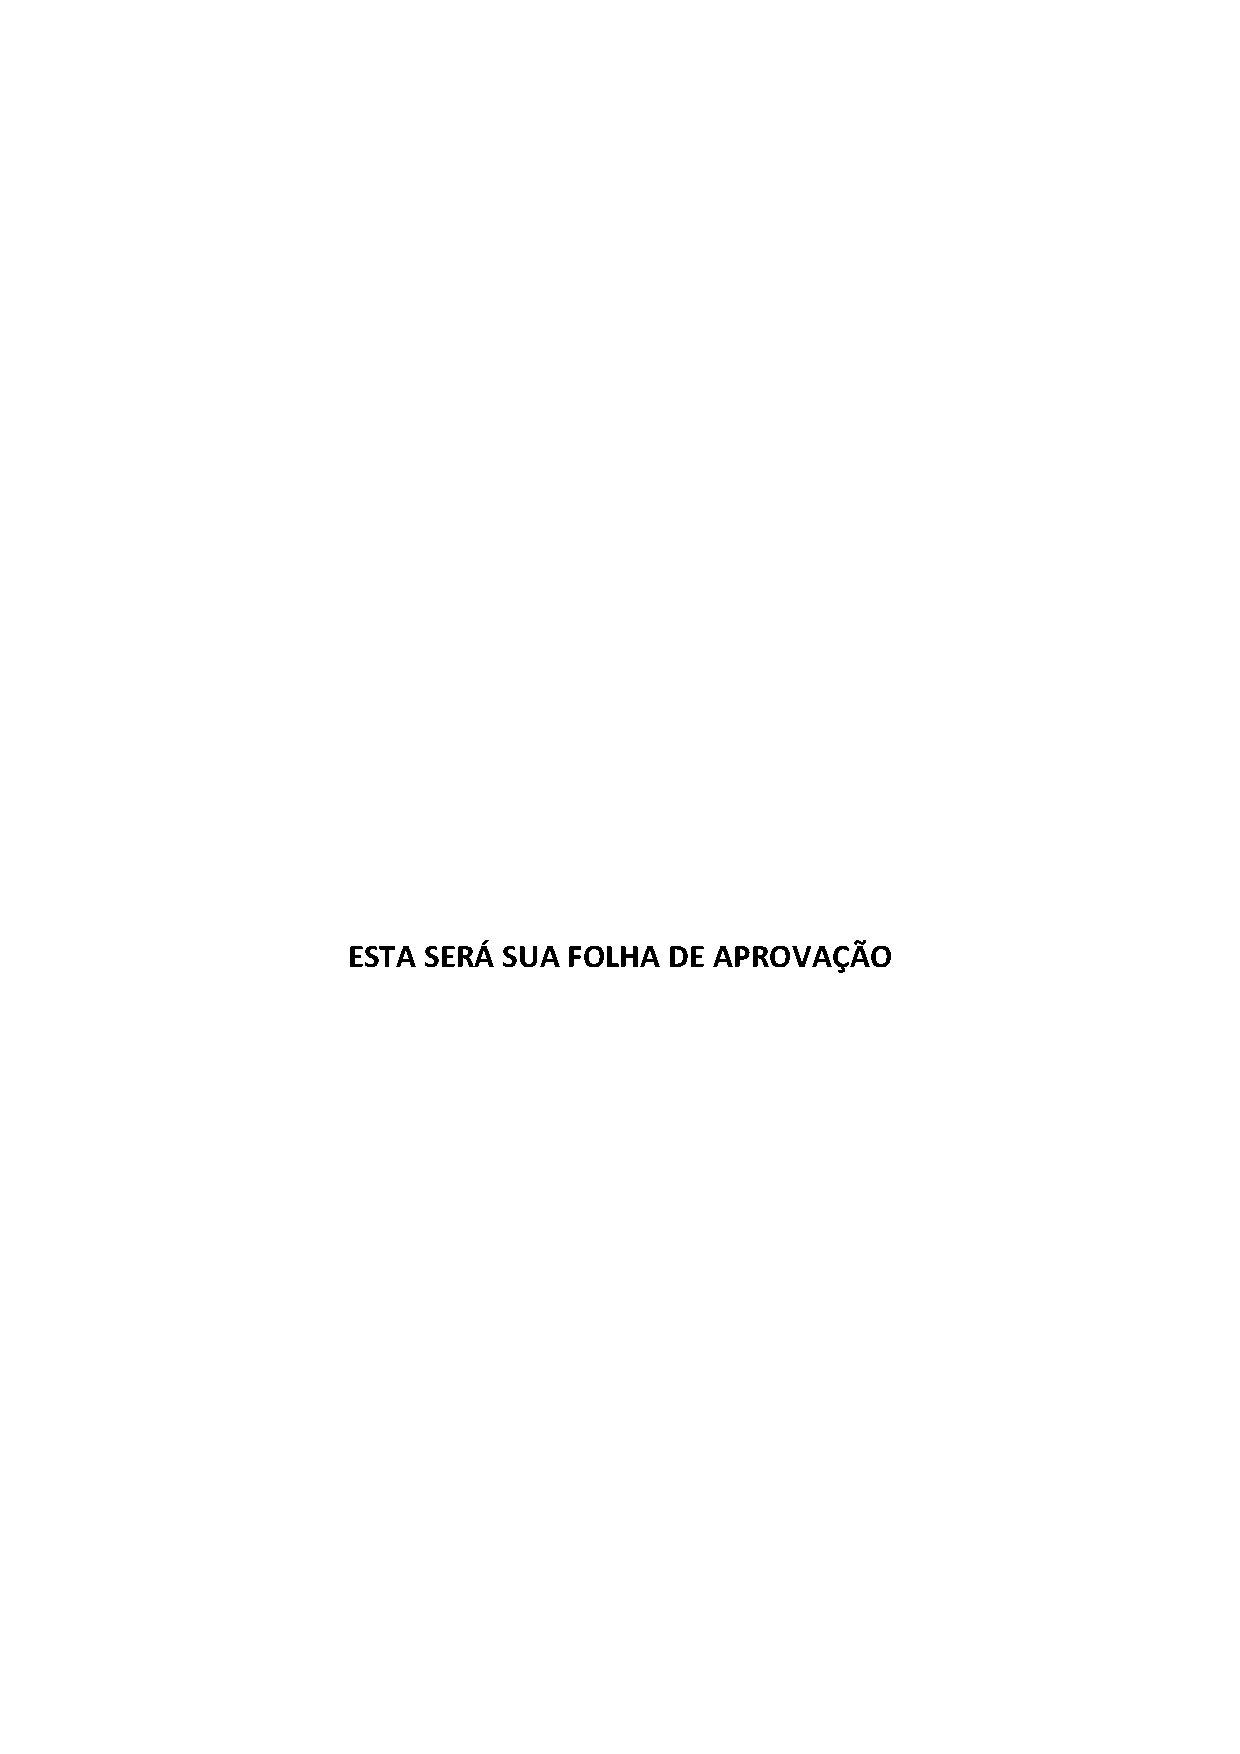
\includepdf[pages=-]{anexos/aprovacao.pdf}

\setlength{\ABNTEXsignwidth}{12cm}

%--------------------------------------------------------------------------------
% Está comentado pelo mesmo motivo da ficha catalográfica 
%--------------------------------------------------------------------------------
%\begin{folhadeaprovacao}
%	\begin{center}
%	    {\ABNTEXchapterfont\bfseries\large\imprimirinstituicao}
%	    \vspace*{\fill}
%
%	    {\ABNTEXchapterfont\bfseries\large FOLHA DE APROVAÇÃO}
%	    \vspace*{\fill}
%
%	    {\ABNTEXchapterfont\bfseries\large\imprimirautor}
%
%	    \vspace*{\fill}\vspace*{\fill}
%	    {\ABNTEXchapterfont\bfseries\large\imprimirtitulo}
%	    \vspace*{\fill}
%
%	    {\hspace{.45\textwidth}
%		\begin{minipage}{.5\textwidth}
%			\SingleSpacing
%			\ABNTEXchapterfont\imprimirpreambulo \\ \\
%
%			{\ABNTEXchapterfont\imprimirorientadorRotulo~\imprimirorientador\par}
%			{\ABNTEXchapterfont\imprimircoorientadorRotulo~\imprimircoorientador\par}
%
%		\end{minipage}%
%	    \vspace*{\fill}}
%	\end{center}
%
%	\vspace*{\fill}	
%	
%	\begin{center}
%			 \ABNTEXchapterfont\large Aprovado em: \_\_\_\_ de \_\_\_\_ de 2017
%	\end{center}

%	\vspace*{\fill}
	
%	\begin{center}
%			 \ABNTEXchapterfont\bfseries\large Banca Examinadora
%	\end{center}
%		
%   \ABNTEXchapterfont\assinatura{Fábio Nelson de Sousa Pereira, Mestre, Universidade Federal do Vale do São Francisco}
%	\ABNTEXchapterfont\assinatura{Jorge Luis Cavalcanti Ramos, Doutor, Universidade Federal do vale do São Francisco}
%  \ABNTEXchapterfont\assinatura{Ricardo Argenton Ramos, Doutor, Universidade Federal do Vale do São Francisco}
%	 \vspace*{\fill}

	 
%\end{folhadeaprovacao}

%--------------------------------------------------------------------------------
% Insere a epígrafe
%--------------------------------------------------------------------------------
%\newpage
%\begin{epigrafe}
%\vspace*{\fill}
%\begin{flushright}
%		\textit{Como aquele que misturou o azul e o amarelo criou o verde, assim como o Yin Yang se opõe e se completa, eu quero conhecer tudo.}\\
%		\textbf{Orochimaru}\\
%		\textbf{Naruto}
%\end{flushright}
%\end{epigrafe}
%--------------------------------------------------------------------------------
% Seção de agradecimentos
%--------------------------------------------------------------------------------
% \begin{agradecimentos}
	
% \lipsum[2-4]

% \end{agradecimentos}

%--------------------------------------------------------------------------------
% Insere a segunda epígrafe
%--------------------------------------------------------------------------------
% \begin{epigrafe}
%     \vspace*{\fill}
% 	\begin{flushright}
% 		Se pude enxergar a tão grande distância, foi subindo nos ombros de gigantes.\\
% 		 \vspace{\baselineskip}
% 		\textbf{Isaac Newton}\\
% 		\textbf{Carta à Robert Hooke, 1676}
% 	\end{flushright}
% \end{epigrafe}



%--------------------------------------------------------------------------------
% Seção de resumos
%--------------------------------------------------------------------------------
% resumo em português
\setlength{\absparsep}{18pt} % ajusta o espaçamento dos parágrafos do resumo
\begin{resumo}

A copa do mundo de futebol de robôs (\textit{RoboCup Soccer}) procura fomentar as pesquisas acerca de robótica e inteligência artificial fornecendo um problema padrão capaz de avaliar teorias, algoritmos e arquiteturas de agentes. O projeto da \textit{RoboCup} é dividida em várias ligas, desde robôs humanoides até a liga de simulação 2D. O desenvolvimento deste trabalho tem como objetivo a continuidade da criação do FutVasf2D como time oficial da Universidade Federal do Vale do São Francisco (UNIVASF) em campeonatos de futebol de robô na liga de simulação 2D. Alguns times que competem ou competiram em campeonatos da liga fornecem código-fonte de times, chamados de times bases, a fim facilitar o desenvolvimento de novos times para novos competidores. É o caso dos times HELIOS, do Japão, que fornece o time base HELIOS Base, ou o WrightEagle, da China, que fornece o WrightEagleBASE, utilizado neste projeto. Tais times são desenvolvidos com estratégias simples para que possam ser melhoradas pelas novas equipes. Através do algoritmo de aprendizado por reforço \textit{Q-Learning}, utilizando dados obtidos do ambiente a partir dos sensores visual, acústico e físico, o agente deve tomar decisões a fim de alcançar melhor resultado na posição de defesa entre diversas ações, como: (1) mover-se para uma melhor posição; (2) marcar um jogador adversário; (3) interceptar a bola e (4) bloquear avanço do jogador com posse de bola.

 \textbf{Palavras-chave}: Futebol de Robôs, Aprendizado por reforço, \textit{Q-Learning}, \textit{RoboCup Simulation 2D}, Defesa.

\end{resumo}

%---------------------------------------------------------------------------------
% resumo em inglês
\begin{resumo}[Abstract]
\begin{otherlanguage*}{english}

The robot soccer world cup (RoboCup Soccer), looks for foment researches about robotics and artificial intelligence providing a default problem capable of evaluate theories, algorithms and architecture of agents. The RoboCup project is divide in various leagues, from humanoid robots to the 2D simulation league. The development of this work has as objective the continuity of the creation of FutVasf2D as official team of Federal University of São Francisco Valley (UNIVASF) at robot soccer championships of 2D simulation league. Some teams which competed or compete in championships from this league provide source codes of teams, called base teams, with the end to ease the development of new teams for new competitors. This is the case of HELIOS, from Japan, which provides the HELIOS Base, or WrightEagle, from China, which provides the WrightEagleBASE, used in this project. These teams are developed with simple strategies so the new team can improve it.Through the reinforcement learning algorithm Q-Learning,  using data obtained from the environment that come from visual, acoustic and physical sensors, the agent must take decisions to get the best results in defense position between diverse actions, like: (1) move to a better position; (2) mark a opponent; (3) intercept the ball e (4) block the player that own the ball from advance.
	
	\vspace{\onelineskip}

	\noindent
	\textbf{Key-words}: \textit{Robot Soccer, Reinforcement Learning, Q-Learning, RoboCup Simulation 2D, Defense}.

\end{otherlanguage*}
\end{resumo}


%---------------------------------------------------------------------------------
% Insere lista de ilustrações
%---------------------------------------------------------------------------------
\begin{KeepFromToc} % Este comando evita que todas as seções dentro dele de apareçam no sumário
\pdfbookmark[0]{\listfigurename}{lof}
\listoffigures
%\addcontentsline{toc}{chapter}{Lista de Figuras}
\cleardoublepage


%---------------------------------------------------------------------------------
% Insere lista de tabelas
%---------------------------------------------------------------------------------
\pdfbookmark[0]{\listtablename}{lot}
\listoftables
\cleardoublepage

%---------------------------------------------------------------------------------
% Ajusta lista de código - alterar de figures para códigos - by @Gabrielr2508
%---------------------------------------------------------------------------------
\makeatletter
\let\l@listing\l@figure
\def\newfloat@listoflisting@hook{\let\figurename\listingname}
\makeatother

%---------------------------------------------------------------------------------
% Insere lista de códigos - by @leolleocomp
%---------------------------------------------------------------------------------
\listoflistings

\end{KeepFromToc}

%---------------------------------------------------------------------------------
% Insere lista de abreviaturas e siglas
%---------------------------------------------------------------------------------
\begin{siglas}
	\item[CBR] Competição Brasileira de Robótica
    \item[CMAC] Computador Aritmético de Modelo Cerebelar
    \item[DCBD] Descoberta de Conhecimento em Base de Dados 
    \item[HAQL] \textit{Q-Learning} Acelerado Heuristicamente
    \item[HFO] Ofensa de Meio Campo
    \item[KDD] Descoberta de Conhecimento em Base de Dados, do inglês \textit{Knowledge Discovery in Databases}
    \item[MDP] Processo de Decisão Markoviano
    \item[PIBIC] Programa Institucional de Bolsas de Iniciação Científica 
    \item[QRL] Aprendizado por Reforço Qualitativo
    \item[QSR] Raciocínio Espacial Qualitativo
    \item[RPROP] \textit{Backpropagation} Resiliente
    \item[SARSA] Estado-Ação-Recompensa-Estado-Ação
    \item[UNIVASF] Universidade Federal do Vale do São Francisco
	    
\end{siglas}

%---------------------------------------------------------------------------------
% Insere o sumario
%---------------------------------------------------------------------------------
\pdfbookmark[0]{\contentsname}{toc} 
\tableofcontents*
\cleardoublepage
